\documentclass[12pt, a4paper]{article}

\usepackage{amsmath}
\usepackage{array}
\usepackage{amsmath}
\usepackage[portuguese]{babel}
\usepackage{chngpage}
\usepackage{float}
\usepackage[a4paper, margin=2cm]{geometry}
\usepackage{graphicx}
\usepackage{hyperref}
\usepackage{listings}
\usepackage{setspace}
\usepackage{xcolor}

\lstdefinestyle{codestyle}{
    commentstyle=\color{teal},
    keywordstyle=\color{blue},
    numberstyle=\ttfamily\color{gray},
    stringstyle=\color{red},
    basicstyle=\ttfamily\footnotesize,
    breakatwhitespace=false,
    breaklines=false,
    keepspaces=true,
    numbers=none,
    showspaces=false,
    showstringspaces=false,
    showtabs=false,
    tabsize=4
}
\lstset{style=codestyle}

\title{\Huge \textbf{Computação Gráfica \\ \Large Trabalho Prático -- Fase II}}
\date{30 de março 2025}
\author{Grupo 3}

\begin{document}

\begin{center}
    
\includegraphics[width=0.25\textwidth]{res/cover/EE-C.eps}
\end{center}

\chardef\_=`_
\onehalfspacing
\setlength{\parskip}{\baselineskip}
\setlength{\parindent}{0pt}
\def\arraystretch{1.5}

{\let\newpage\relax\maketitle}
\maketitle
\thispagestyle{empty}

\vspace*{\fill}

\begin{adjustwidth}{-2cm}{-2cm} % These values only need to be large enough to center the table
    \begin{center}
        \begin{tabular}{>{\centering}p{0.25\textwidth}
                        >{\centering}p{0.25\textwidth}
                        >{\centering}p{0.25\textwidth}
                        >{\centering\arraybackslash}p{0.25\textwidth}}
            
\includegraphics[width=3.5cm]{res/cover/A104437.png} &
            
\includegraphics[width=3.5cm]{res/cover/A104348.png} &
            
\includegraphics[width=3.5cm]{res/cover/A90817.png} &
            
\includegraphics[width=3.5cm]{res/cover/A104179.png} \\

            Ana Oliveira & Humberto Gomes & Mariana Cristino & Sara Lopes \\
            A104437      & A104348        & A90817           & A104179
        \end{tabular}
    \end{center}
\end{adjustwidth}

\pagebreak

\begin{abstract}
    \textbf{\color{red} TODO - resumo}
\end{abstract}

\section{Transformações}

Um dos objetivos desta fase do trabalho prático é a possibilidade de aplicar transformações de
translação, rotação e escala às entidades na cena. Estas podem ser especificadas no ficheiro XML
como se apresenta no exemplo abaixo:

\lstset{language=xml}
\begin{lstlisting}

<group>
    <transform>
		<translate            x="1" y="2" z="3" />
        <rotate    angle="90" x="0" y="0" z="1" />
		<scale                x="1" y="2" z="1" />
    </transform>
    <models>
        <model file="modelo.3d" />
    </models>
</group>
\end{lstlisting}

Neste exemplo, a todos os modelos em \texttt{<models>} devem ser aplicadas, por esta ordem, uma
translação pelo vetor $(1, 2, 3)$, uma rotação de 90º pelo eixo $z$, e uma escala vertical por um
fator de duas vezes. Para calcular as matrizes associadas a cada uma destas transformações, as
funções \texttt{glm::translate}, \texttt{glm::rotate}, \texttt{glm::scale} são utilizadas.
\cite{glm-transform} Estas são semelhantes às funções \texttt{glTranslate}, \texttt{glRotate} e
\texttt{glScale} \cite{gl-transforms}, respetivamente, mas devolvem a matriz de transformação
calculada, em vez de modificarem as matrizes do estado interno do OpenGL. Outra diferença é que o
ângulo dado à função \texttt{glm::rotate} deve ser passado em radianos, sendo necessária uma
conversão do valor em graus presente na descrição XML da cena.

Para compor estas operações, as matrizes geradas pela \texttt{glm} são multiplicadas pela ordem em
que as transformações surgem no ficheiro XML. No exemplo anterior, onde $T$ é a matriz da
translação, $R$ a matriz de rotação, e $S$ a matriz de escala, as coordenadas no mundo dos pontos do
modelo devem ser multiplicadas pela matriz $W$ abaixo, originando as coordenadas no mundo do modelo
transformado:

$$
W = T R S
$$

Para desenhar as entidades no ecrã, é necessário também ter em conta a matriz da câmara, $C$, o
produto entre a matriz de projeção e a matriz de vista. Ademais, como os grupos na cena formam uma
hierarquia, é necessário considerar as transformações dos ascendentes de um grupo para o desenhar.
Assim, para desenhar a cena, usa-se uma \emph{stack} de matrizes, inicializada com a matriz da
câmara. Depois, para cada grupo aninhado, calcula-se o produto entre a matriz no topo do
\emph{stack} e a matriz de transformação do grupo, e esta matriz calculada é adicionada ao topo da
\emph{stack}. Quando se termina o desenho do grupo, é removida a matriz do topo da \emph{stack}. No
exemplo abaixo, mostra-se a \emph{stack} de matrizes durante o desenho de um grupo na hierarquia da
cena:

\begin{figure}[h]
    \begin{minipage}{0.5\textwidth}
        \centering
        \begin{tabular}{|>{\centering\arraybackslash}m{3cm}|}
            \hline \\
            \hline $C \cdot T_1 \cdot T_3 \cdot T_4$ \\
            \hline $C \cdot T_1 \cdot T_3$ \\
            \hline $C \cdot T_1$ \\
            \hline $C$ \\
            \hline
        \end{tabular}
    \end{minipage}
    \begin{minipage}{0.5\textwidth}
        \centering
        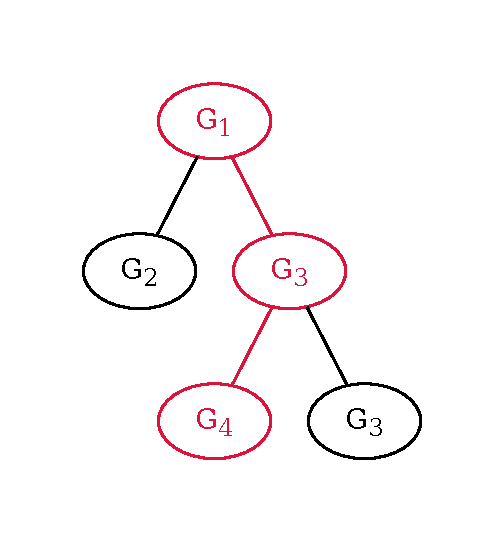
\includegraphics[width=0.6\textwidth]{res/phase2/SceneGraph.pdf}
    \end{minipage}
    \caption{\emph{Stack} de matrizes associada ao desenho de um grupo numa cena hierárquica.}
\end{figure}

\section{Modelo estático do sistema solar}

\textbf{\color{red} TODO - sistema solar}

\section{Extras}

\textbf{\color{red} TODO - extras}

\section{Resultados obtidos}

\textbf{\color{red} TODO - resultados}

\section{Conclusão e Trabalho Futuro}

\textbf{\color{red} TODO - conclusão}

\begingroup
\section{Bibliografia}
\renewcommand{\section}[2]{}

\begin{thebibliography}{9}
    \bibitem{glm-transform}
        ``GLM\textunderscore EXT\textunderscore matrix\textunderscore transform''. GLM 0.9.9 API
        documentation. Accessed: Mar. 27, 2025. [Online.] Available:
        \url{https://glm.g-truc.net/0.9.9/api/a00247.html}
    \bibitem{gl-transforms}
        ``OpenGL (R) 2.1, GLX, and GLU Reference Pages ''. Khronos Registry.
        Accessed: Mar. 27, 2025. [Online.] Available:
        \url{https://registry.khronos.org/OpenGL-Refpages/gl2.1}
\end{thebibliography}
\endgroup

\end{document}
